% presentation
\documentclass{beamer}

\usetheme{Warsaw}

% rus lang
\usepackage[main=russian,english]{babel}

% insert images
\usepackage{wrapfig}
\usepackage{graphicx}

% declare operator
\DeclareMathOperator*{\argmin}{argmin} % thin space, limits underneath in displays
\newcommand{\at}[2][]{#1|_{#2}}

% alrorithm
\usepackage{algorithm2e}
\usepackage{algorithm}
\usepackage{algpseudocode}
% \usepackage{algorithmic}

% math
\newtheorem{rustheorem}{Теорема}
\usepackage{amsmath}
\DeclareMathOperator{\sign}{sign}
\DeclareMathOperator{\K}{K}

\title[Линейные методы классификации]{Лекция 4. Линейные методы классификации}
\subtitle{Основы интеллектуального анализа данных}
\author{Полузёров Т. Д.}
\institute{БГУ ФПМИ}
\date{}

\begin{document}
	
	\begin{frame}
		\titlepage
	\end{frame}
	
	\begin{center}
		\frametitle{Структура лекции}
		\tableofcontents	
	\end{center}
	
	\section{Общие идеи}
	
	\subsection{Постановка задачи}
	
	\begin{frame}
		\frametitle{Бинарная классификация}
		Рассмотрим задачу бинарной классификации, $X=(x_1, ..., x_{\ell}) \in \mathbb{X}, Y \in \mathbb{Y} = \{-1, 1\}$
		
		\vspace{5pt}
		
		Модель для классификации
		\[
		a(x, \theta) 
		= \sign f(x, \theta)
		=
		\begin{cases}
			1,& f(x) > 0 \\
			-1,& f(x) < 0
		\end{cases}
		\]
		- где $f(x, \theta)$
		будем называть \textbf{дискриминантной функцией}.
		
		\vspace{5pt}
		
		Множество точек $x$ где $f(x, \theta) = 0$ - \textbf{разделяющая поверхность}.
		
		\vspace{5pt}
		
		Задача состоит в настройке параметров $\theta$ в функции $f(x, \theta)$ по выборке $(X, Y)$
	\end{frame} 
	
	\begin{frame}
		\frametitle{Пример}
		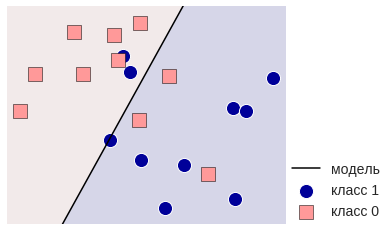
\includegraphics[width=1\textwidth]{img/bin_class}
	\end{frame}

	\begin{frame}
		\frametitle{Отступ}
		
		Величина 
		\[
		M_i(\theta) = y_i f(x_i, \theta)
		\]
		
		 - \textbf{отступ} (margin) классификатора $a(x, \theta) = \sign f(x, \theta)$ относительно объекта $x_i$.
		
		\vspace{5pt}
		
		Если $M_i(\theta) < 0$ то алгоритм $a$ допускает ошибку на объекте $x_i$. 
		
		%\vspace{15pt}
		
		%\textbf{Чем больше} $M_i(\theta)$ \textbf{тем правильнее} и надежнее классификация.
		
		\begin{figure}
			\centering
			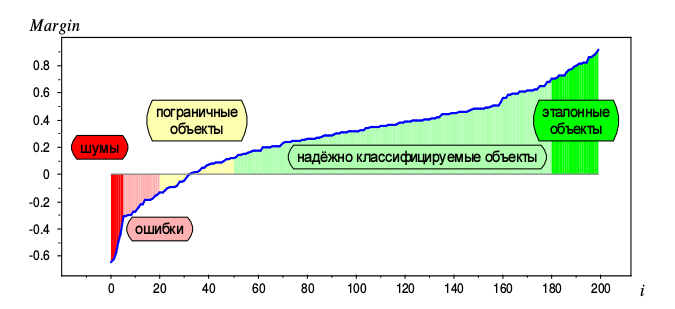
\includegraphics[width=0.8\textwidth]{img/margin}  
		\end{figure}
		
	\end{frame}
	
	\subsection{Оценка сверху эмперического риска}
	
	\begin{frame}
		\frametitle{Функция потерь}
		Требуется подобрать параметры $\theta$ при которых классификатор $a$ допускает как можно меньше ошибок:
		
		\[
		Q(a, X) = \frac{1}{\ell} \sum_{i=1}^{\ell} [M_i(\theta) < 0] \rightarrow \min_{\theta}
		\]
		
		Однако в таком виде $Q$ - кусочно постоянная функция
		
		\vspace{15pt}
		
		Идея - мажорирование (оценка сверху) индикатора ошибки $[M_i(\theta) < 0]$ с помощью "удобной" функцией потерь $\mathcal{L}(M_i)$:
		
		\[
		Q(a, X) = \frac{1}{\ell} \sum_{i=1}^{\ell} [M_i(\theta) < 0]
		\le
		\widetilde{Q}(a, X) = \frac{1}{\ell} \sum_{i=1}^{\ell} \mathcal{L}(M_i(\theta))
		\]
	\end{frame}
	
	\begin{frame}
		\frametitle{Популярные функции потерь}
		
		\begin{columns}
			\begin{column}{0.4\textwidth}
				\begin{enumerate}
					\item $[M < 0]$ - индикатор ошибки
					\item $(1 - M)^2$ - квадратичная
					\item $(1 - M)_{+}$ - \textbf{кусочно линейная (Hinge loss)}
					\item $\frac{2}{1 + e^M}$ - сигмоидная
					\item $\log_2(1 + e^{-M})$ - \textbf{логистическая}
					\item $e^{-M}$ - экспоненциальная
				\end{enumerate}
			\end{column}
			\begin{column}{0.6\textwidth}
				\centering
				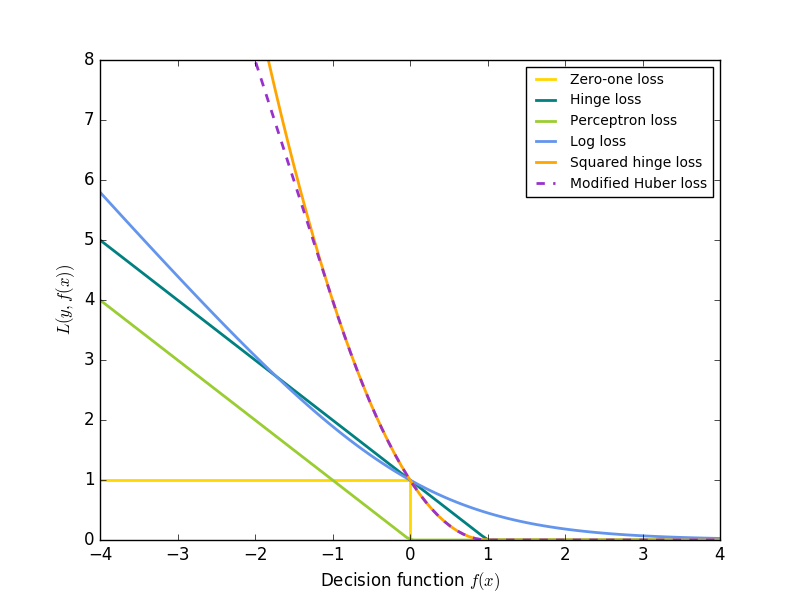
\includegraphics[width=1.15\textwidth]{img/loss_func.png}	
			\end{column}
		\end{columns}
	\end{frame}
	
	\begin{frame}
		\frametitle{Функция потерь и совместное распределение}
		Пусть множество $(\mathbb{X} \times \mathbb{Y})$ - вероятностное пространосво. Имея выборку $(X, Y)$ и предполагаемый вид совместной плотности $p(x, y; \theta)$, применим метод максимального правдоподобия
		
		\[
		L(\theta) = \prod_{i=1}^{\ell} p(x_i, y_i; \theta) \rightarrow \max_{\theta}
		\]
		
		\[
		\ln L = \sum_{i=1}^{\ell} \ln p(x_i, y_i; \theta) \rightarrow \max_{\theta}
		\]
		
		\[
		- \ln p(x_i, y_i; \theta) = \mathcal{L}(y_i f(x_i, \theta))
		\]
		
		По виду плотности $p(x, y; \theta)$ восстанавливается $f$ и $\mathcal{L}$. И обратно, используя некоторые разделяющую поверхность и функцию потерь - предполагаем определенное распределение в данных.
	\end{frame}
	
	\subsection{Линейная модель}
	
	\begin{frame}
		\frametitle{Линейная модель}
		
		Случай $f(x, \omega) = \langle x, \omega \rangle$ - класс линейных моделей классификации.
		
		\[
		a(x, \omega) = \sign \langle x, \omega \rangle
		\]
		
		Разделяющая поверхность $\sign \langle x, \omega \rangle = 0$ является гиперплосткостью в $\mathbb{R}^{n}$. Причем объекты по одну сторону от гиперплосткости относятся к одному классу, по другую - к другому.
	\end{frame}

	
	\begin{frame}
		\frametitle{Метод обучения}
		Метод минимизации мажорированного эмперического риска 
		
		\[
		\widetilde{Q}(a, X) = \sum_{i=1}^{\ell} \mathcal{L}(\langle x_i, \omega \rangle y_i) \rightarrow \min_{\omega}
		\]
		
		Необходимое условие минимума:
		\[
		\frac{\partial Q}{\partial \omega} = \sum_{i=1}^{\ell}  x_i y_i \mathcal{L}^{'}(\langle x_i, \omega \rangle y_i) = 0
		\]
	\end{frame}
	
	\begin{frame}
		\frametitle{Модель нейрона МакКаллока-Питтса}
				
		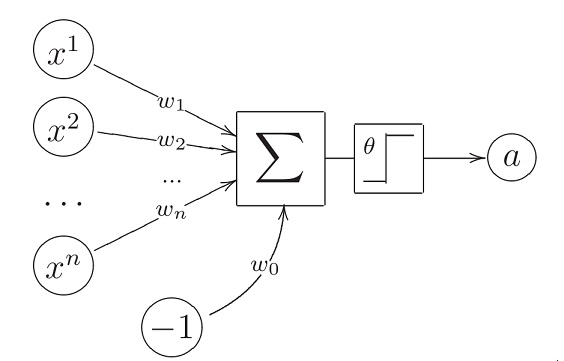
\includegraphics[width=\textwidth]{img/mk_pits.jpg}
	\end{frame}
	
	\section{Логистическая регрессия}
	
	\subsection{Обоснование модели}
	
	\begin{frame}
		\frametitle{Логистическая регрессия}
		Логистическая регрессия (Logistic regression) - линейный алгоритм бинарной классификации.
		
		\vspace{15pt}
		
		При выполнении достаточно сильных предположений обладает свойствами:
		\begin{itemize}
			\item оптимальный байесовский классификатор
			\item однозначно определена функция потерь
			\item возможность оценивать вероятности классов
		\end{itemize}
		
		\vspace{15pt}
		
		Пусть $(\mathbb{X}\times \mathbb{Y}) = (\mathbb{R}^{n} \times \{-1, 1\})$ - вероятностное пространтсво с плотностью $p(x, y)$. Выборка $(X, Y)$ получена из этого распределения.
	\end{frame}
	
	\begin{frame}
		\frametitle{Экспонентный класс распределений}
		Плотность $p(x), x \in \mathbb{R}^{n}$ называется экспонентной, если
		\[
		p(x) = \exp(c(\delta) \langle \theta, x \rangle + b(\delta, \theta) + d(x, \delta))
		\]
		где $\theta$ -параметр сдвига, $\delta$ - масштаба, $b, c, d$ - произвольные числовые функции.
		
		\vspace{15pt}
		
		Принадлежат к классу экспонентных:
		\begin{itemize}
			\item Равномерное, Нормальное, Гамма
			\item Гипергеометрическое, Пуассоновское, Биномиальное
			\item и другие
		\end{itemize}
	\end{frame}
	
	\begin{frame}
		\frametitle{Обоснование линейной модели}
		
		\begin{rustheorem}
		\textbf{Если} функции правдоподобия $p(x | y) $ принадлежат экспонентному классу, причем параметры $d$ и $\delta$ одинаковы, а отличаются только параметры сдвига $\theta$, 
		
		\textbf{то}:
		\begin{enumerate}
			\item оптимальный байесовский классификатор является линейным%: $a(x) = \sign \langle \omega, x \rangle$
			\item апостериорная вероятность $p(y | x) = \sigma(\langle \omega, x \rangle y)$
		\end{enumerate}
		
		где $\sigma(z) = \frac{1}{1 + e^{-z}}$ - сигмоидная функция, $\sigma(-z) = 1 - \sigma(z)$
		\end{rustheorem}	
	\end{frame}
	
	\begin{frame}
		\frametitle{Сигмоидная функция}
		
		\begin{figure}
			\centering
			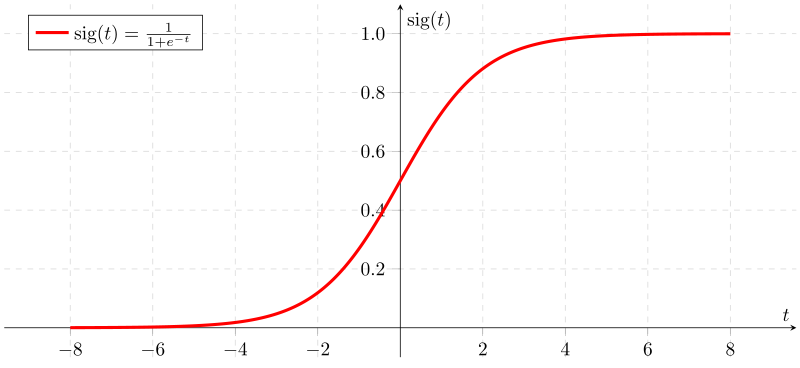
\includegraphics[width=1\textwidth]{img/sigmoida}
		\end{figure}
	\end{frame}
	
	\begin{frame}
		\frametitle{Модель оценки вероятностей}
		Построим модель которая оценивает не сами метки классов, а \textbf{вероятности} принадлежности к ним.
		
		\[
		b(x, \omega) = P(+1 | x) = \sigma(\langle \omega, x \rangle)
		\]
		
		Другими словами, в каждой точке $x$ величина $y \sim Bernoulli(\sigma(\langle \omega, x \rangle))$
		
		\vspace{15pt}
		
		Задача классификации решается путем выбора порога $t \in [0, 1]$. И тогда итоговый классификатор имеет вид:
		
		\[
		a(x, t) = \sign (a(x, \omega) - t)
		\]
		
	\end{frame}
	
	\subsection{Поиск решения}
	
	\begin{frame}
		\frametitle{Метод максимального правдоподобия}
		С учетом вероятностной постановки задачи, воспользуемся \textbf{методом максимального правдоподобия}:
		
		\[
		L(\omega) = \prod_{i=1}^{\ell} p(y_i | x_i) = 
		\prod_{i=1}^{\ell} \sigma(\langle \omega, x_i \rangle y_i)
		\rightarrow \max_{\omega}
		\]
		
		\[
		\ln L(\omega) 
		= \sum_{i=1}^{\ell} \ln \sigma(\langle \omega, x_i \rangle y_i)
		=
		\]
		\[
		= 
		- \sum_{i=1}^{\ell} \ln(1 + e^{-y_i \langle \omega, x \rangle}) \rightarrow \max_{\omega}
		\]
		
		-совпадает с логистической функция потерь 
		\[
		Q(\omega) = \sum_{i=1}^{\ell} \ln (1 + e^{-M_i}) \rightarrow \min_{\omega}
		\]
	\end{frame}
	
	\begin{frame}
		\frametitle{Решение оптимизационной задачи}
		Имеем
		
		\[
		Q(\omega) = \sum_{i=1}^{\ell} \ln (1 + e^{- y_i \langle \omega, x \rangle}) \rightarrow \min_{\omega}
		\]
		
		Аналитического решения нет, поэтому применяются градиентные методы
		\[
		\nabla Q(\omega) = \sum_{i=1}^{\ell} x_i y_i \sigma(- \langle \omega, x_i \rangle)
		\]
	\end{frame}
	
	\begin{frame}
		\frametitle{Логистическая регрессия}
		Получена модель \textbf{логистической регрессии} $b: \mathbb{X} \rightarrow [0, 1]$
		\[
		b(x) = \sigma(\langle x, \omega \rangle)
		\]
		При обучении используется логистическая функция потерь
		\[
		\mathcal{L}(y, a) = \ln(1 + e^{-y_i \langle \omega, x \rangle})
		\]
		
		Выбирая порог $t \in [0, 1]$ получаем классификатор
		\[
		a(x) = [b(x) > t]
		\]
		
	\end{frame}
	
	\section{Метод опорных векторов}
	
	\subsection{Линейно разделимая выборка}
	
	\begin{frame}
		\frametitle{Случай линейно разделимой выборки}
		
		По выборке $(X, Y)$ будем строить классификатор вида
		\[
		a(x, \omega) = \langle x, \omega \rangle - \omega_0
		\]
		
		и предположим, что выборка $(X, Y)$ линейна разделима. То есть найдутся такие веса $\omega^{*}$, что 
		\[
		Q(\omega^{*}) = \frac{1}{\ell} [y_i \cdot a(x_i, \omega^{*}) < 0] = 0
		\]
		
		Однако такое решение $\omega^{*}$ не единственное. Идея состоит в распоряжении этой свободой с умом.
	\end{frame}
	
	\begin{frame}
		\frametitle{Максимизация отступа}
		Среди всех подходящих разделяющих гиперплоскостей выберем ту, которая максимально удалена от "граничных" объектов.
		
		\vspace{5pt}
		
		\begin{columns}
			\begin{column}{0.4\textwidth}
				\centering
				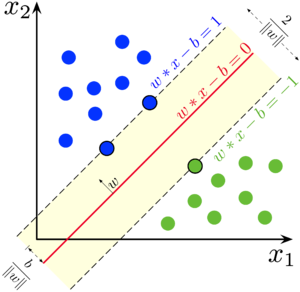
\includegraphics[width=\textwidth]{img/svm.png}		
			\end{column}
			\begin{column}{0.6\textwidth}
				Вследствие линейной разделимости
				
				$\exists \omega, \omega_0 : \{x: -1 < \langle \omega, x \rangle - \omega_0 < 1\}$
				-~полоса между классами.
				
				\vspace{5pt}
				
				Выберем наиболее широкую из всех доступных
				\[
				\begin{cases}
					||\omega||^2 \rightarrow \min \\
					M_i(\omega) \ge 1, &  i=1, ..., \ell
				\end{cases}
				\]
			\end{column}
		\end{columns}
	\end{frame}
	
	\subsection{Линейно неразделимая выборка}
	
	\begin{frame}
		\frametitle{Линейно неразделимая выборка}
		В случае линейно неразделимой выборки смягчим требования
		\[
		\begin{cases}
			\frac{1}{2}||\omega||^2 + \alert{C \sum_{i=1}^{\ell} \xi_i} \rightarrow \min \\
			M_i(\omega) \ge 1 - \alert{\xi_i},  i=1, ..., \ell \\
			\alert{\xi_i \ge 0}, i=1, ..., \ell
		\end{cases}
		\]
		
		Требование можно упростить
		\[
			\begin{cases}
				\xi_i \ge 0\\
				\xi_i \ge 1 - M_i(\omega)\\
				\sum_{i=1}^{\ell} \xi_i \rightarrow \min
			\end{cases}	
			&
			\Rightarrow
			&
			\xi_i = (1 - M_i(\omega))_{+}
		\]

		Итог - задача безусловной оптимизации
		\[
		\frac{1}{2}||\omega||^2 + C \sum_{i=1}^{\ell} (1 - M_i(\omega))_{+} \rightarrow \min_{\omega}
		\]
		где $C$ - гиперпарамер алгоритма
		
	\end{frame}
	
	\begin{frame}
		\frametitle{Метод опорных векторов}
		Получен \textbf{метод опорных векторов} (Support Vector Machine, SVM), где
		\[
		a(x) = \sign \left( \langle x, \omega \rangle \right)
		\]
		\[
		\mathcal{L}(y, a) = (1 - M_i(\omega))_{+}
		\]
		Т.е. линейный классификатор с квадратичной регуляризацией, обученный по функции потерь Hinge loss
	\end{frame}
	
	\begin{frame}
		\frametitle{Двойственная задача}
		По теореме Каруша-Куна-Такера, исходная задача эквивалентна двойственной задаче поиска седловой точки функции Лагранжа
		\[
		\mathcal{L}(\omega, \alert{\lambda, \eta}) = 
		\frac{1}{2} ||\omega||^2 
		- \sum_{i=1}^{\ell} \alert{\lambda_i} (M_i(\omega) - 1)
		- \sum_{i=1}^{\ell} \xi_i (\alert{\lambda_i} + \alert{\eta_i} - C)
		\]
		
		Приравнивая частные производные $\mathcal{L}$ по $\omega, \omega_0, \xi$ к нулю
		\[
		\begin{cases}
			\omega = \sum_{i=1}^{\ell} \lambda_i y_i x_i \\
			\sum_{i=1}^{\ell} \lambda_i y_i = 0 \\
			\eta_i + \lambda_i = C, i=1, ..., \ell
		\end{cases}
		\]
	\end{frame}
	
	\begin{frame}
		\frametitle{Типы объектов}
		 При условии
		 \[
		 \begin{cases}
		 	\eta_i + \lambda_i = C, i=1, ..., \ell \\
		 	\eta_i \ge 0, \lambda_i \ge 0
		 \end{cases}
		 \]
		 
		 Существуют три ситуации
		 \begin{enumerate}
		 	\item $\lambda_i = 0, \eta_i = C, \xi_i = 0, M_i \ge 1$
		 	- \textbf{неинформативный}  объект, классифицируется правильно и не влияет на $\omega$
		 	
		 	\item $0 < \lambda_i < C, 0 < \eta_i < C, \xi_i = 0, M_i = 1$
		 	- \textbf{опорный} объект, классифицируется правильно и лежит на разделяющей полосе
		 	
		 	\item $\lambda_i = C, \eta_i = 0, \xi_i > 0, M_i < 1$
		 	- \textbf{опорный нарушитель}, либо неверно классифицируется, либо лежит внутри разделяющей полосы
		 \end{enumerate}
	\end{frame}
	
	\begin{frame}
		\frametitle{Альтернативный вид классификатора}
		Подставляя ограничения в лагранжиан, переходим к двойственной задаче с двойственными переменными $\lambda$
		\[
		\begin{cases}
			- \sum_{i=1}^{\ell} \lambda_i + 
			\frac{1}{2} \sum_{i=1}^{\ell} \sum_{j=1}^{\ell}
			\lambda_i \lambda_j y_i y_j \langle x_i, x_j \rangle
			\rightarrow \min_{\lambda} \\
			
			0 \le \lambda_i \le C, i=1, ..., \ell \\
			
			\sum_{i=1}^{\ell} \lambda_i y_i = 0
		\end{cases}
		\]
		
		 Получив решение $\lambda$, параметры классификатора равны
		\[
		\begin{cases}
			\omega = \sum_{i=1}^{\ell} \lambda_i y_i x_i \\
			\omega_0 = \langle x_i, \omega \rangle - y_i, & \forall i: \lambda_i > 0, M_i = 1
		\end{cases}
		\]
		
		И итоговый классификатор имеет вид
		\[
		a(x) = \sign \left( \sum_{i=1}^{\ell} \lambda_i y_i \langle x, x_i \rangle - \omega_0 \right)
		\]
	\end{frame}
	
	\subsection{Трюк с ядром}
	
	\begin{frame}
		\frametitle{Трюк с ядром}
		Идея состоит в переходе от исходного призакового пространства $\mathbb{X}$ в другое $\mathbb{H}$ где, быть может, выборка является линейно разделимой, посредством $\psi: \mathbb{X} \rightarrow \mathbb{H}$. 
		
		Это выливается в использование вместо $\langle \psi (x_i), \psi (x_j) \rangle$ некоторого ядра $K(x_i, x_j)$
		
		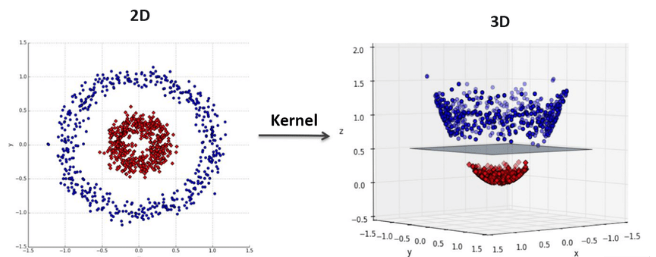
\includegraphics[width=1\textwidth]{img/kernel_trick.png}
	\end{frame}
	
	\begin{frame}
		\begin{columns}
			\begin{column}{0.5\textwidth}
				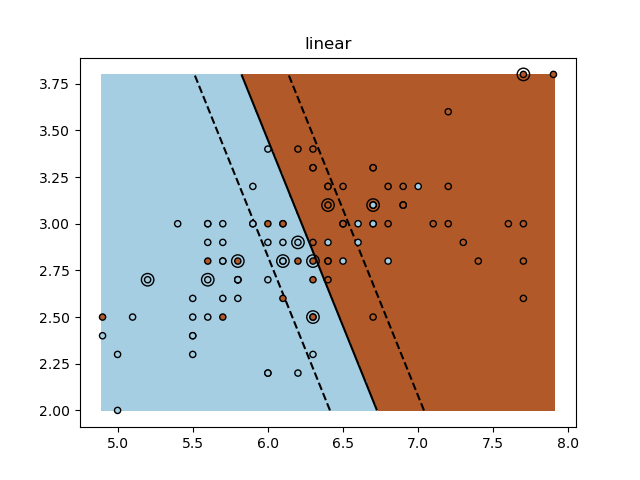
\includegraphics[width=1\textwidth]{img/svm_kernels_1}
				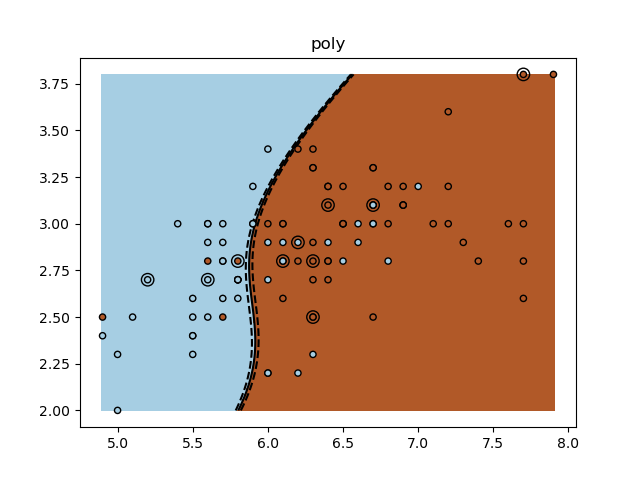
\includegraphics[width=1\textwidth]{img/svm_kernels_2}
			\end{column}
			\begin{column}[t]{0.5\textwidth}
				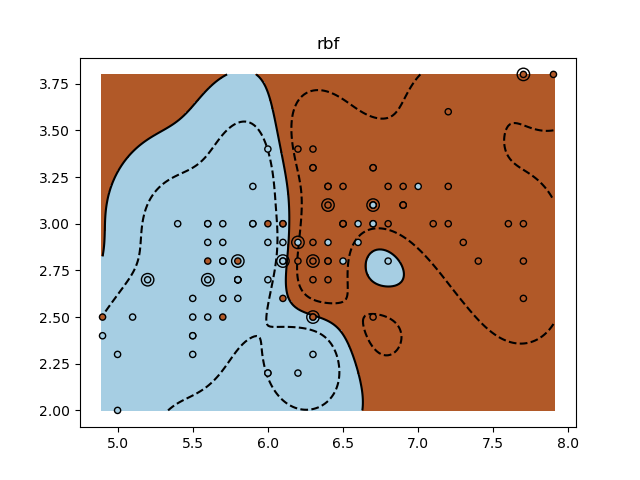
\includegraphics[width=1\textwidth]{img/svm_kernels_3}
			\end{column}			
		\end{columns}
	\end{frame}
	
	\begin{frame}
		\frametitle{Заключение}
		
		\begin{itemize}
			\item Линейный классификатор - модель нейрона
			\item Аппроксимация пороговой функции потерь
			\item Оценка вероятностей с помощью логистической регрессии
			\item SVM - очень сильный алгоритм классификации благодаря трюку с ядром
		\end{itemize}
	\end{frame}
\end{document}